\begin{frame}{Featureless Machine Learning}
\begin{itemize}
  \item Works with Raw data (converted into numeric form)
  \item Keeps semantics
\end{itemize}

Notes:
\begin{itemize}
  \item vector size might be an issue
  \item found techniques to reduce vector size
  \item embedding
  \item dimensionality reduction
\end{itemize}

\end{frame}

\begin{frame}{Feature-Based Machine Learning}
  \begin{itemize}
    \item Feature Extraction
    \item Does not keeps semantics
    \item Smaller Vector size
    \item complexity increases with number of features
  \end{itemize}
  
  Feature Selection:
  \begin{itemize}
    \item manuelle
    \item automatic
    \item Irrelevant features: overfitting
    \item Redundant features: correlation, decrease robustness
    \item based on statistical parameters
    \item wrapper method (based on the accuracy of the model)
    \item Evaluate Feature importance (Random Forest Model feature\_importances)
  \end{itemize}
\end{frame}



\begin{frame}{ML: Moldel Performances}
  \begin{itemize}
    \item Depends on the dataset
    \item Accuracy of the model (shallow)
    \item AUC (Area Under the Curve)
    \item ROC curve (Receiver Operating Characteristics)
    \item Cross-Validation (helps to avoid overfitting and selection bias problem)
  \end{itemize}
\end{frame}


\begin{frame}{ML: Moldels }
  Classification / Linear Regression
  \begin{itemize}
    \item Hyperplan that separates two classes
    \item Space with as many dimensions as features
  \end{itemize}
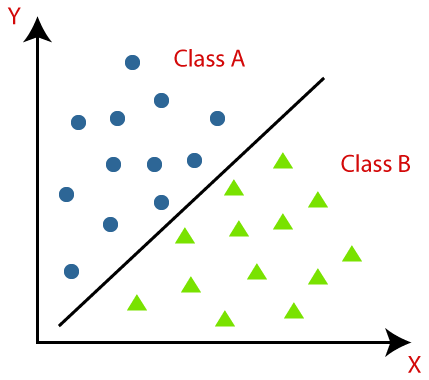
\includegraphics[width=.5\textwidth]{class.png}
\end{frame}

\begin{frame}{ML: Moldels }
  Random forest model\\
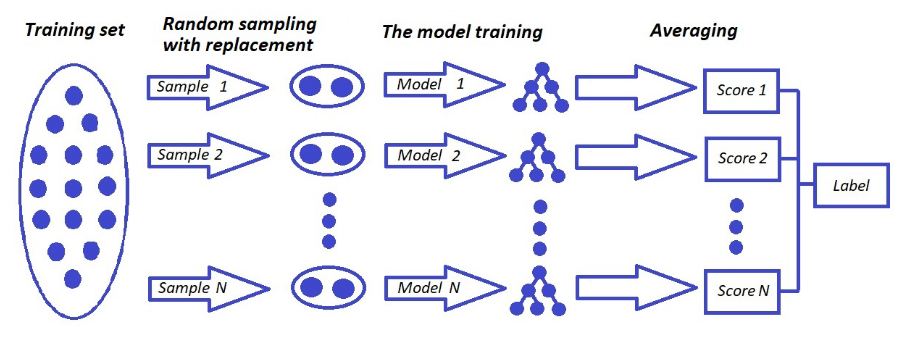
\includegraphics[width=.8\textwidth]{forest1.png}\\
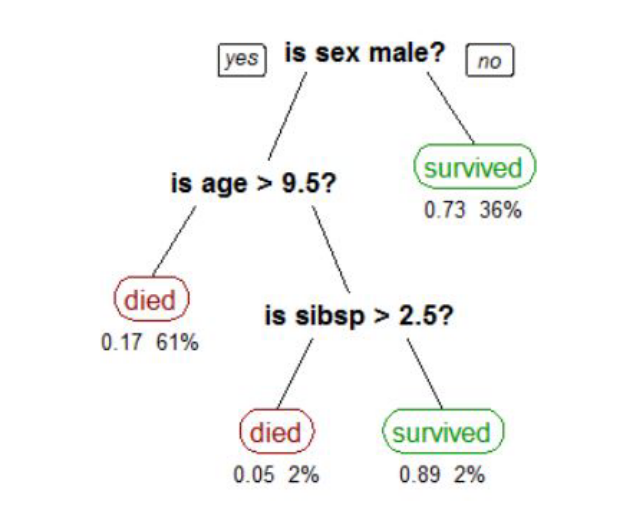
\includegraphics[width=.4\textwidth]{forest2.png}
\end{frame}

\begin{frame}{ML: Moldels }
  Gradient Boosting model
  \begin{itemize}
    \item takes previous errors into account
  \end{itemize}
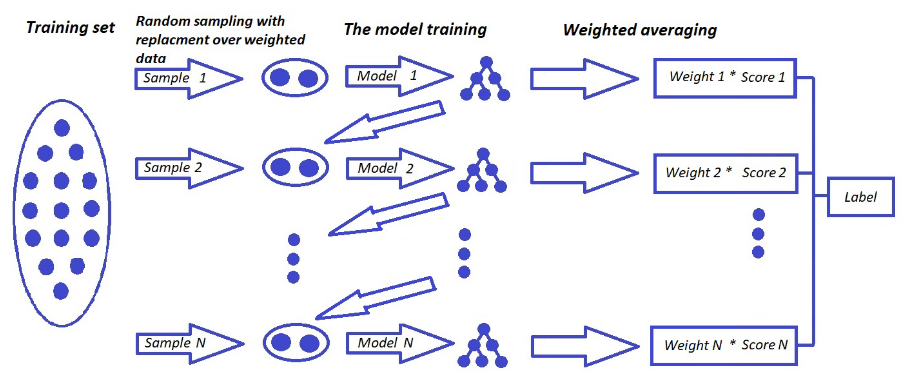
\includegraphics[width=\textwidth]{gradient.png}
\end{frame}

\begin{frame}{Model Evaluation}
  \begin{itemize}
    \item Performances
    \begin{itemize}
      \item Forest \& Boosting: way better than Linear/Classification
      \item Boosting marginally better than Forest
    \end{itemize}
    \item Training time
    \begin{itemize}
        \item Linear and Gradient (way) faster than Forest
    \end{itemize}
    \item Prediction time
    \begin{itemize}
        \item Ramdom Forest: slowest
        \item Linear/Classification: fastest
    \end{itemize}
  \end{itemize}
\end{frame}

%    \includegraphics[width=\textwidth]{analyserisque.png}

%    \includegraphics[width=\textwidth]{archie.png}
%    \begin{minipage}[t]{0.3\textwidth}
%    \end{minipage}
